\chapter{Gestión de Unidades de Aprendizaje}
\section{Consultar de Unidades de Aprendizaje}
Para consultar Unidades de Aprendizaje el Jefe de Innovación Educativa consulta un Plan de Estudios en la pantalla \hyperlink{consultarS}{\textit{Consultar Planes de Estudios}}:\\
\begin{figure}[!hbtp]
    \centering
    \hypertarget{consultarS}{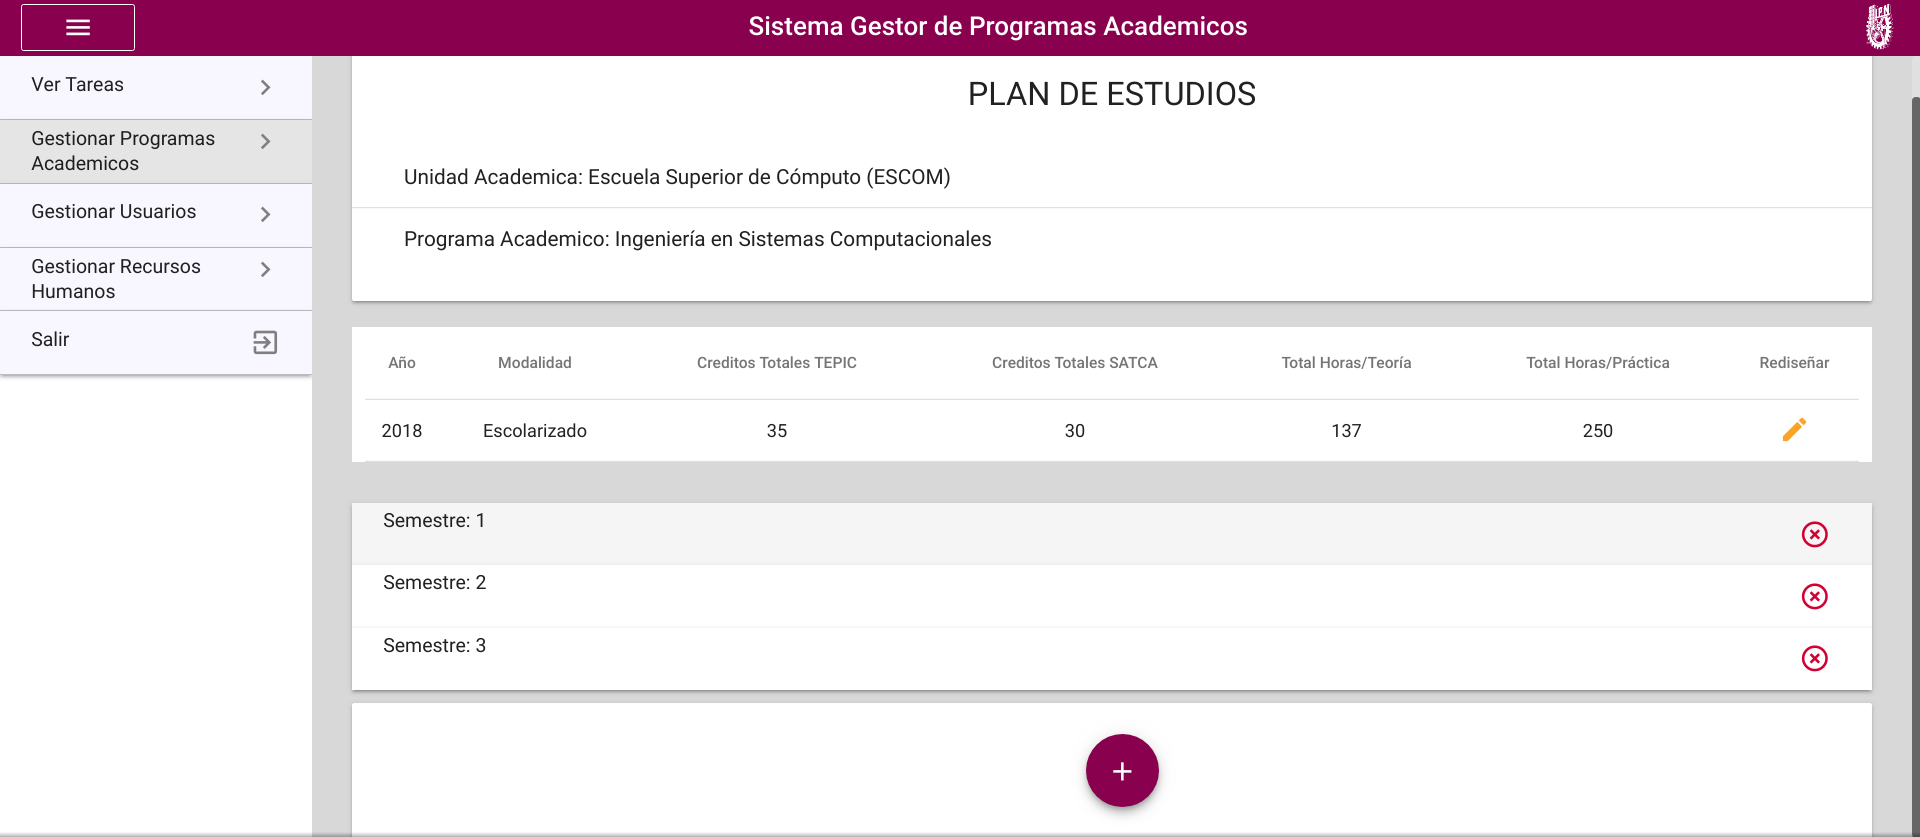
\includegraphics[width=0.7\linewidth]{images/GUA/consultarS}}
    \caption{Pantalla Consultar Plan de Estudios}
    \label{consultarS}
\end{figure}
Una vez en esta pantalla el usuario selecciona un semestre y este se expande desplegando las Unidades de Aprendizaje que tiene asociadas en la siguiente pantalla \hyperlink{consultarUA}{\textit{Consultar Planes de Estudios}}:\\
\begin{figure}[!hbtp]
    \centering
    \hypertarget{consultarUA}{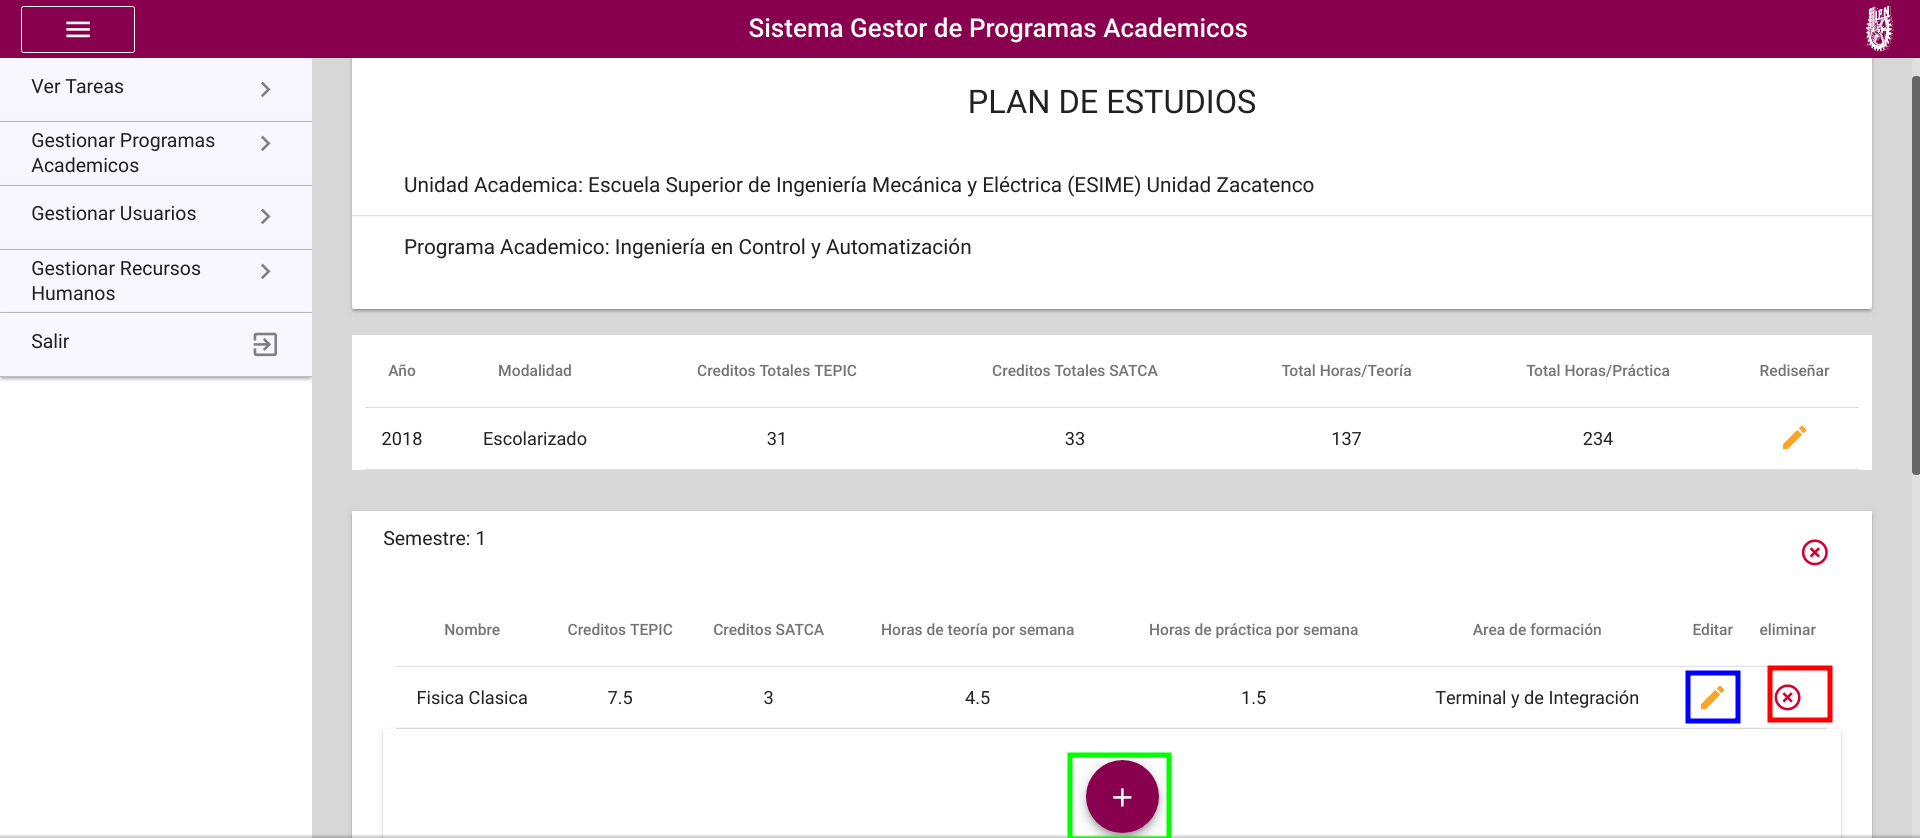
\includegraphics[width=0.7\linewidth]{images/GUA/consultarUA}}
    \caption{Pantalla Consultar Plan de Estudios Semestre expandido}
    \label{consultarUA}
\end{figure}
En esta ultima pantalla podemos realizar las tareas relacionadas a la gestión de Unidades de Aprendizaje, presionando en los iconos en recuadros de colores para registrar(verde), editar(azul) y eliminar (rojo).
\newpage
\section{Registrar Unidades de Aprendizaje}
Cuando el Jefe de Innovación Educativa presiona el icono de \IUbutton{+} en el recuadro verde en la pantalla \hyperlink{consultarUA}{\textit{Consultar Planes de Estudios}} lo lleva a la siguiente pantalla la siguiente pantalla \hyperlink{registrarUA}{\textit{Registrar Unidad de Aprendizaje}}:\\
\begin{figure}[!hbtp]
    \centering
    \hypertarget{registrarUA}{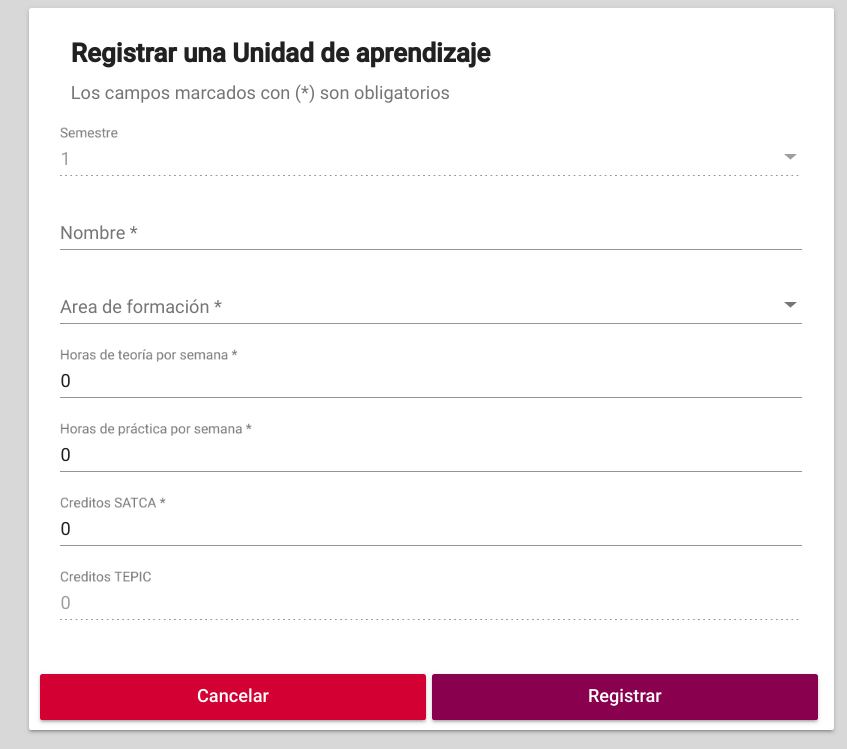
\includegraphics[width=0.7\linewidth]{images/GUA/registrarUA}}
    \caption{Pantalla Registrar Unidad de Aprendizaje}
    \label{registrarUA}
\end{figure}
\newpage
Durante el registro el sistema puede lanzar los siguientes mensajes
\begin{figure}[!hbtp]
    \centering
    \hypertarget{invalidoR}{
\includegraphics[width=0.7\linewidth]{images/GUA/invalido}}
    \caption{Campo invalido: aparece cuando el formato o el tipo de dato es incorrecto}
    \label{invalidoR}
\end{figure}
\begin{figure}[!hbtp]
    \centering
    \hypertarget{requeridoR}{
\includegraphics[width=0.7\linewidth]{images/GUA/requerido}}
    \caption{Campo requerido: aparece cuando un campo obligatorio se dejo vacio}
    \label{requeridoR}
\end{figure}
\begin{figure}[!hbtp]
    \centering
    \hypertarget{exito}{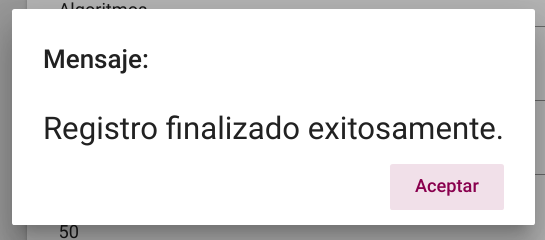
\includegraphics[width=0.7\linewidth]{images/GUA/exito}}
    \caption{Regisro Exitoso: aparece cuando su registro finaliza sin errores}
    \label{exito}
\end{figure}
\begin{figure}[!hbtp]
    \centering
    \hypertarget{cancelarR}{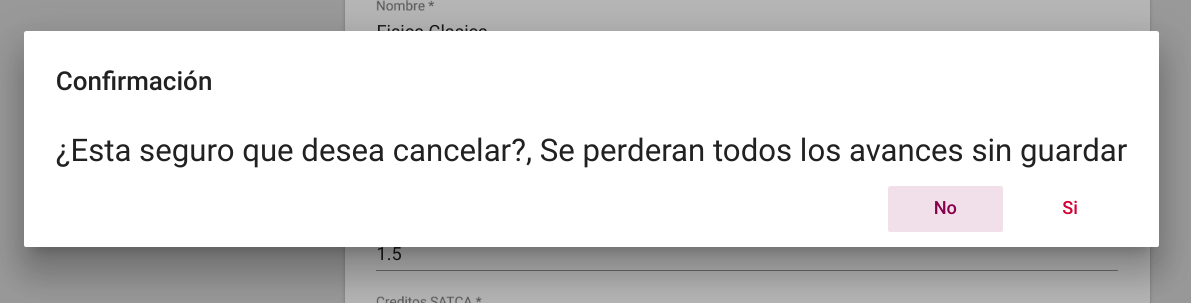
\includegraphics[width=0.7\linewidth]{images/GUA/cancelar}}
    \caption{Cancelación: este mensaje nos permite finalizar la operacion sin guardar}
    \label{cancelarR}
\end{figure}
\newpage
\section{Editar Unidades de Aprendizaje}
Cuando el Jefe de Innovación Educativa presiona el icono de \IUbutton{+} en el recuadro verde en la pantalla \hyperlink{consultarUA}{\textit{Consultar Planes de Estudios}} lo lleva a la siguiente pantalla la siguiente pantalla \hyperlink{editarUA}{\textit{Editar Unidad de Aprendizaje}}:\\
\begin{figure}[!hbtp]
    \centering
    \hypertarget{editarUA}{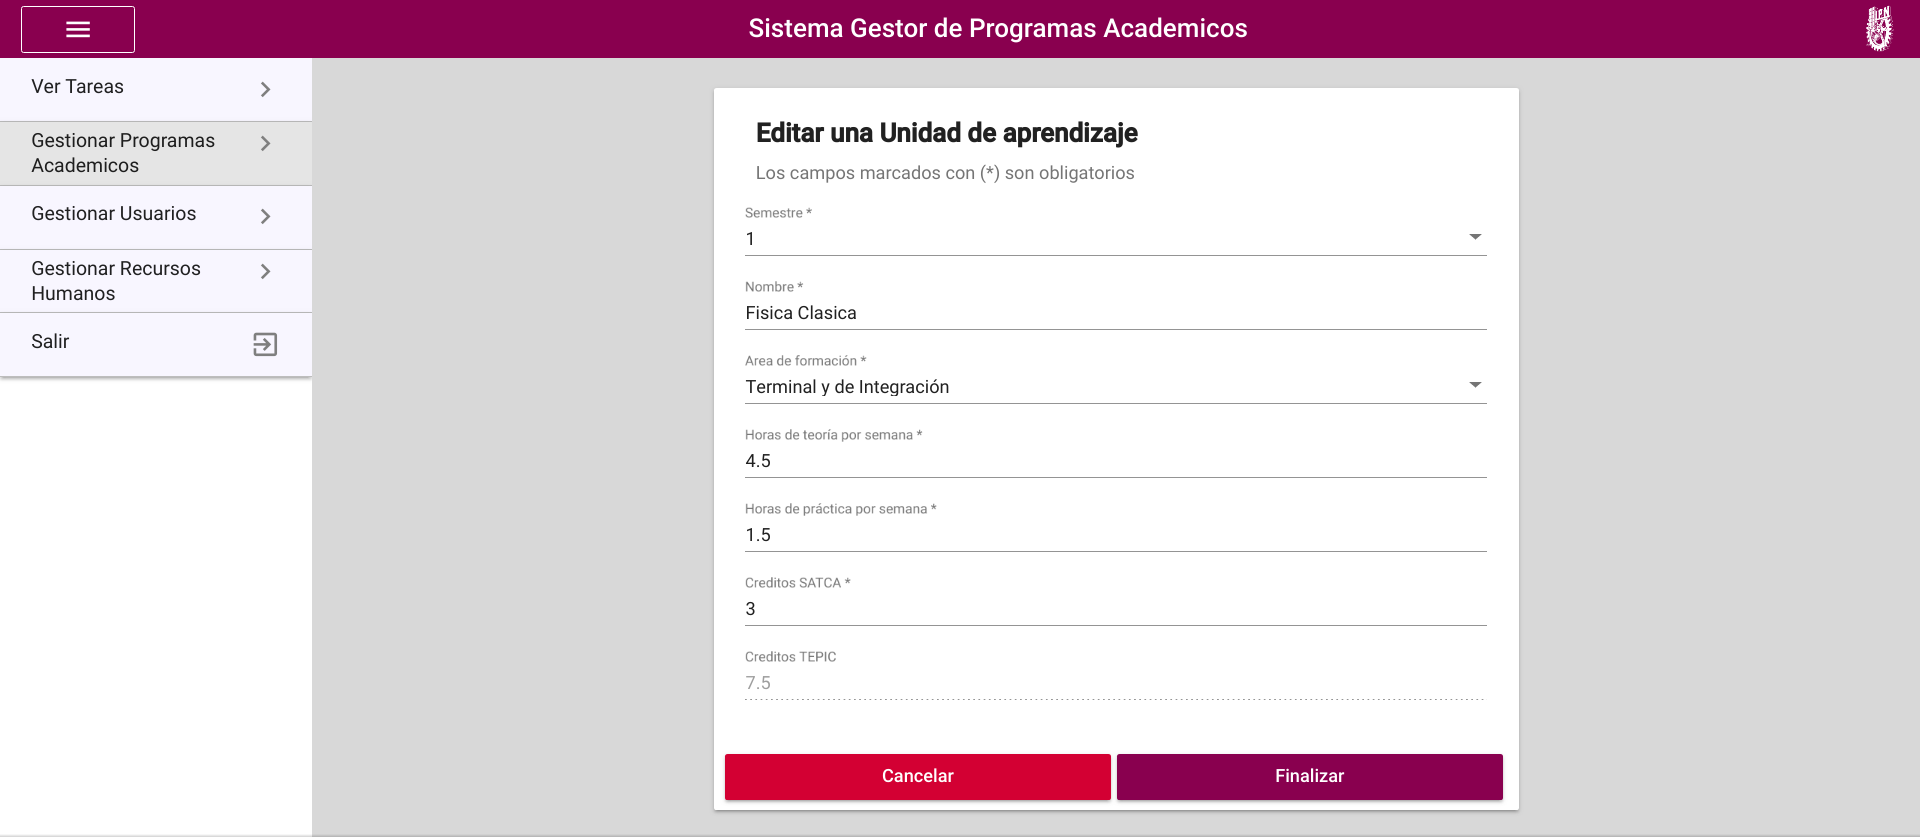
\includegraphics[width=0.7\linewidth]{images/GUA/editarUA}}
    \caption{Pantalla Editar Unidad de Aprendizaje}
    \label{editarUA}
\end{figure}
Durante la edición el sistema puede lanzar los siguientes mensajes:\\
\begin{figure}[!hbtp]
    \centering
    \hypertarget{invalidoE}{
\includegraphics[width=0.7\linewidth]{images/GUA/invalido}}
    \caption{Campo invalido: aparece cuando el formato o el tipo de dato es incorrecto}
    \label{invalidoE}
\end{figure}
\begin{figure}[!hbtp]
    \centering
    \hypertarget{requeridoE}{
\includegraphics[width=0.7\linewidth]{images/GUA/requerido}}
    \caption{Campo requerido: aparece cuando un campo obligatorio se dejo vacio}
    \label{requeridoE}
\end{figure}
\begin{figure}[!hbtp]
    \centering
    \hypertarget{modificacion}{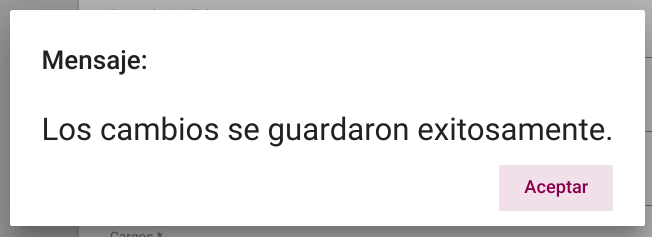
\includegraphics[width=0.7\linewidth]{images/GUA/modificacion}}
    \caption{Modificación exitosa: mensaje puramente de notificación}
    \label{modificacion}
\end{figure}
\begin{figure}[!hbtp]
    \centering
    \hypertarget{cancelarE}{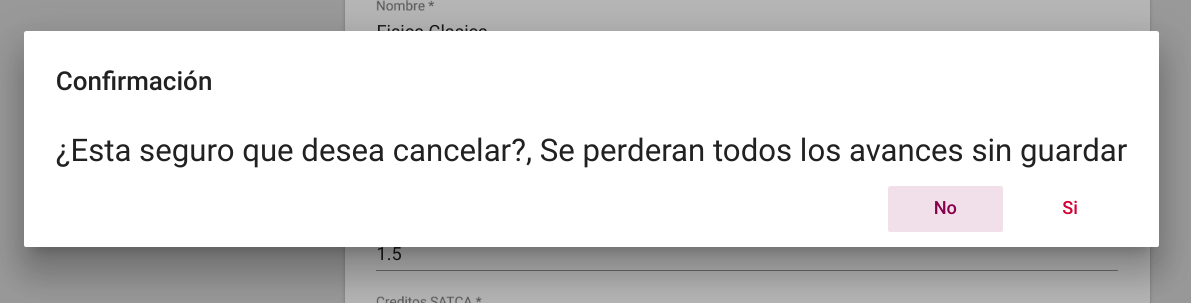
\includegraphics[width=0.7\linewidth]{images/GUA/cancelar}}
    \caption{Cancelación: este mensaje nos permite finalizar la operacion sin guardar}
    \label{cancelarE}
\end{figure}
\newpage
\section{Eliminar Unidades de Aprendizaje}
Cuando el Jefe de Innovación Educativa presiona el icono de \IUbutton{X} en el recuadro rojo en la pantalla \hyperlink{consultarUA}{\textit{Consultar Planes de Estudios}} aparece:\\
\begin{figure}[!hbtp]
    \centering
    \hypertarget{EliminarUA}{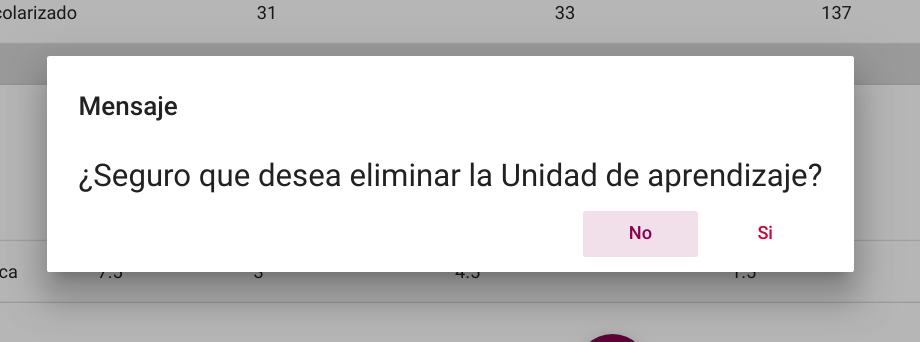
\includegraphics[width=0.7\linewidth]{images/GUA/EliminarUA}}
    \caption{Eliminar Unidad de Aprendizaje: solicita confirmación para eliminar permanentemente una Unidad de Aprendizaje}
    \label{EliminarUA}
\end{figure}